\section{复数的指数形式}\label{009}

\begin{flushright}{\kaishu \textbf{虚}中有\textbf{实}者, 或山穷水尽处, 一折而豁然开朗. - 沈复
『浮生六记』 \\Lesson 5: 最短的捷径就是绕远路,
绕远路才是我的最短捷径.\footnote{\emph{ジョジョの奇妙な冒险 Part7
  スティ-ル・ボ-ル・ラン}.}}\end{flushright}

\begin{tcolorbox}[size=fbox, breakable, enhanced jigsaw, title={极坐标 (polar coordinate)}]

其实在\ref{005}\nameref{005}中已经借用了一点极坐标的概念, 这里再正式地介绍一遍.
在平面直角坐标系里, 一个点所在的位置具有两个自由度 (degree of freedom),
因此一般不多不少需要两个独立变量来锚定这个点, 通常我们会有一个点的
$x$-轴坐标和 $y$-轴坐标来表示这个点的位置 $(x,y)$. 当然,
我们也可以在建立坐标系后, 利用和原点的距离 $r$, 和一个方向,
例如【$x$-轴正方向】至【这个点和原点的连线】顺时针方向形成的夹角
$\theta$, 来表示一个点的位置 $(r,\theta)$.

\begin{tcolorbox}[size=fbox, breakable, enhanced jigsaw]
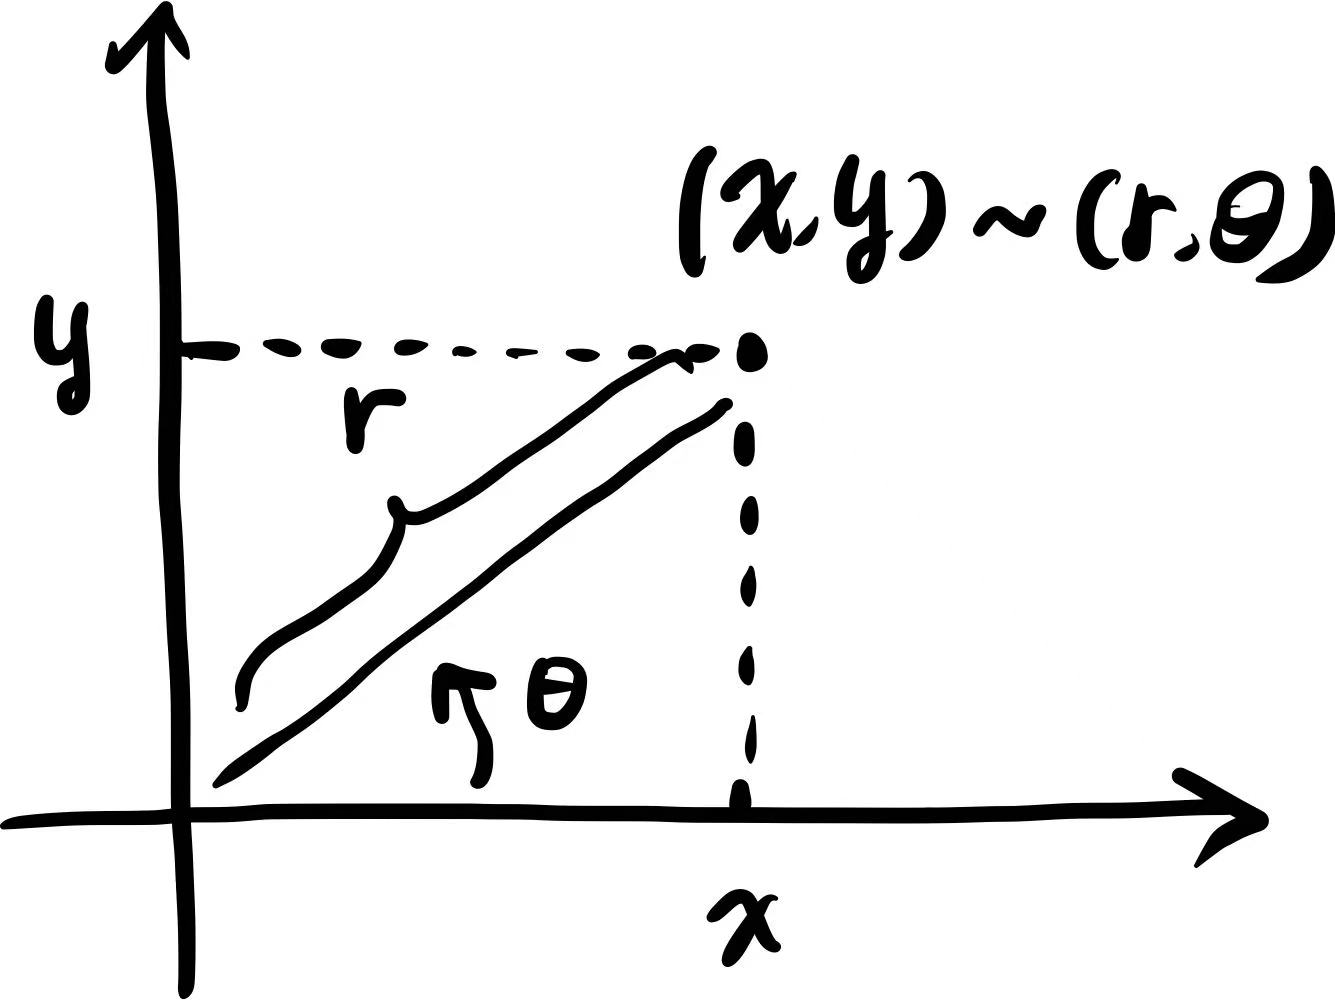
\includegraphics[width=0.5\textwidth]{img/image-20230418112700129.png}

\kaishu{\small 极坐标}
\end{tcolorbox}

不难看出, 存在以下的转换

$\begin{cases}x=r\cos\theta\\y=r\sin\theta\end{cases};\ \begin{cases}r=\sqrt{x^2+y^2}\\\theta=\arctan (y/x)\end{cases}.$

上式中 $\arctan$ 是 $\tan$ 的逆运算, 即
$\tan\theta=y/x\Rightarrow \theta=\arctan (y/x)$, 有时 $\arctan$
也记作 $\tan^{-1}$.

\end{tcolorbox}

\begin{tcolorbox}[size=fbox, breakable, enhanced jigsaw, title={复平面 (complex
plane)}]

考虑实数的时候, 有时我们会想象有一条数轴, 在\ref{001}\nameref{001}和\ref{002}\nameref{002}中,
我们将这条数轴添上了最初离散分布的整数,
然后又补上了似乎没有空隙的有理数, 最后才用全体实数彻底``填满''了.
在\ref{006}\nameref{006}中, 我们研究的对象再次扩展到了复数,
于是一条实轴似乎``放不下''这些复数的存在了, 我们便添加一条额外的,
与之前实数轴垂直的虚数轴, 如此一来便构成了一个复平面.

那么考虑一个复数 $(a+bi)$, 它的实部大小便是 $a$, 虚部大小便是 $b$,
仿照着实二维平面直角坐标系, 我们便可以在复平面上标出 $(a+bi)$
对应的一个点. 既然如此, 我们可以继续仿照着极坐标, 表示出至原点的距离,
以及 $x$-轴正方向到这个点和原点的连线顺时针方向形成的夹角,
这两个量在复平面中分别被称作\textbf{模} (modulus, 合理怀疑有音译成分)
和\textbf{辐角} (argument), 记作

$ | a+bi|=\sqrt{a^2+b^2},~\arg(a+bi)=\arctan (b/a).$

\begin{tcolorbox}[size=fbox, breakable, enhanced jigsaw]
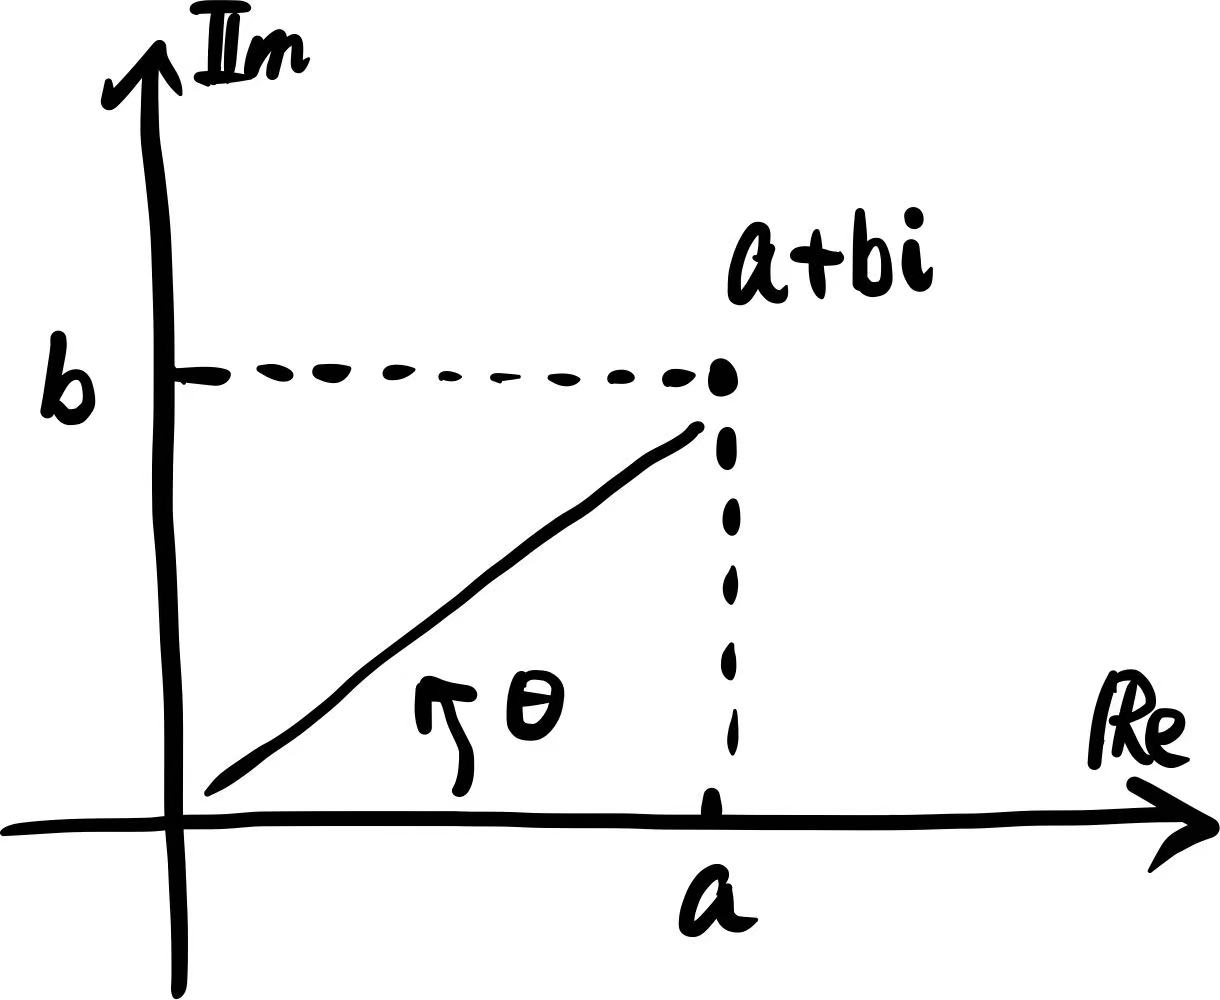
\includegraphics[width=0.5\textwidth]{img/image-20230418112740537.png}

\kaishu{\small 复平面}
\end{tcolorbox}

\begin{newquote}
像, 太像了.\footnote{\emph{让子弹飞}.}
\end{newquote}

若是把模和辐角分别记作 $r$ 和 $\theta$, 则这个复数 $(a+bi)$
便可以表示为

$(a+bi)=r\cos\theta+ir\sin\theta.$

\end{tcolorbox}

\begin{tcolorbox}[size=fbox, breakable, enhanced jigsaw, title={复数的指数形式}]

有那么一点跳脱, 怎么突然扯到指数了呢? 在\ref{002}\nameref{002}中,
其实我们只讨论过指数为有理数的情况, 当然指数是任意实数的情况, 例如
$\sqrt{2}$ , 我们也可以利用 $\sqrt{2}=1.414213...$ 去估算,
或者丢给一个科学计算器; 但是当指数是虚数或者复数时,
似乎情况就不大一样了\ldots 考虑自然常数为底数, 我们从自然常数的定义出发,
\ref{008}\nameref{008}中我们有

$\lim_{n\rightarrow\infty}\left(1+\frac{1}{n}\right)^n\equiv\mathrm{e}.$

不难推出, 对于任意实数 $x$, 有

$\lim_{n\rightarrow\infty}\left(1+\frac{x}{n}\right)^n=\mathrm{e}^x.$

把上面结论推广到虚数,

$\lim_{n\rightarrow\infty}\left(1+\frac{i}{n}\right)^n=\mathrm{e}^i.$

如果上式让您感到不适 (uncomfortable), 您大可用二项式展开 (参见\ref{007}\nameref{007})
来确认一下上述结果的正当性 (validity). 怎么理解这个 $\mathrm{e}^i$ 呢,
不妨来看看它的模和辐角.

在此之前, 我们还需要一些小\textbf{引理} (lemma \footnote{\textbf{公理/假定}
  (axiom/postulate): 默认为真无需证明的陈述. \textbf{定义} (definition):
  准确无歧义的对一个术语的描述. \textbf{定理} (theorem):
  证明为真的大结论. \textbf{引理} (lemma): 为了证明定理的小结论.
  \textbf{推论} (Corollary): 借助定理可简短地证明的结论.
  一本严格的数学书经常会出现前面这些令人畏惧的词,
  类似的还有\textbf{命题} (proposition), \textbf{推测/猜想}
  (conjecture), \textbf{断言} (claim)等等.}, 区别于 llama - 大羊驼,
好冷), 这里没有严谨证明, 仅提供一个思路:

\begin{tcolorbox}[size=fbox, breakable, enhanced jigsaw, title={引理1}]
$\boxed{|(a+bi)^n|=|a+bi|^n}$.
\end{tcolorbox}

\begin{newquote}
当 $n=2$ 时, $(a+bi)^2=a^2-b^2+2abi$. 于是

$\begin{aligned}|(a+bi)^2|=&\sqrt{(a^2-b^2)^2+(2ab)^2}\\=&\sqrt{(a^2+b^2)^2}\\=&\sqrt{(a^2+b^2)}^2\\=&|a+bi|^2.\end{aligned}$

用数学归纳法 (关于数学归纳法, 可以参见\ref{007}\nameref{007}中的一个实例)
便不难得出结论.
\end{newquote}

\begin{tcolorbox}[size=fbox, breakable, enhanced jigsaw, title={引理2}]
$\boxed{\arg((a+bi)^n)=n\cdot\arg(a+bi)}$.
\end{tcolorbox}

\begin{tcolorbox}[size=fbox, breakable, enhanced jigsaw, sidebyside]
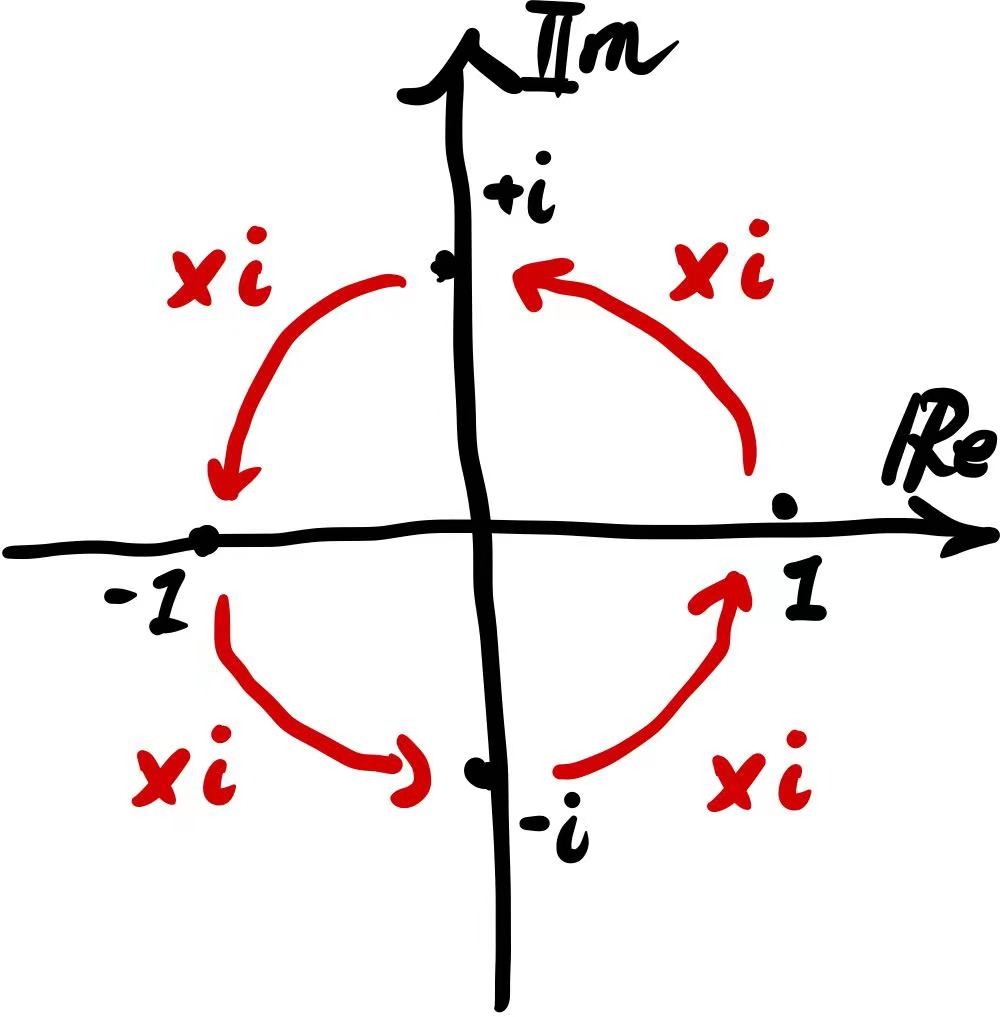
\includegraphics[width=0.9\textwidth]{img/image-20230418114331337.png}
\tcblower
\kaishu{\small 这里需要引入一个新的视角, 我们把复数看作一个``作用'',
将一个复数作用在某一个数 $z$ 上, 在复平面上事实上是将 $z$
对应的点关于原点旋转了. 考虑 $i\times1$, 即将 $i$ 作用到 $1$ 上,
得到了 $i$, 相当于逆时针旋转了 $90^\circ$; 继续作用 $i$, 得到了
$-1$, 相当于又逆时针旋转了 $90^\circ$\ldots{} 于是用 $i$ 作用
$n$ 次, 即作用了 $i^n$, 相当于将其作用对象, 关于原点, 旋转了 $i$
的辐角 $90^\circ$ $n$ 次, 便是旋转了 $n90^\circ$. ( $90^\circ$
用 $\pi/2$ 弧度表述其实会更好, 关于弧度可以参考\ref{005}\nameref{005},
下文若无额外说明, 角度皆用弧度制).

这个结论可以推广到其他任意复数, 便有了上述结论.}
\end{tcolorbox}

事实上, 利用辐角和模来表述一个复数, 上述两则引理可以总结成一条:

\begin{tcolorbox}[size=fbox, breakable, enhanced jigsaw, title={引理1+2}]
$\boxed{\left[r(\cos\theta+i\cos\theta)\right]^n=r^n(\cos n\theta+i\sin n\theta)}$.
\end{tcolorbox}

那么来看 $\mathrm{e}^i$ , 它的模

$\begin{aligned} |\mathrm{e}^i|=&\left|\lim_{n\rightarrow\infty}\left(1+\frac{i}{n}\right)^n\right|\\ =&\lim_{n\rightarrow\infty}\left|\left(1+\frac{i}{n}\right)^n\right|\\ =&\lim_{n\rightarrow\infty}\sqrt{1+\frac{1}{n^2}}^n\\ =&\lim_{n\rightarrow\infty}\left(1+\frac{1}{n^2}\right)^{n/2}\\ =&\lim_{n\rightarrow\infty}\left[\left(1+\frac{1}{n^2}\right)^{n^2}\right]^{1/2n}=\lim_{n\rightarrow\infty}\mathrm{e}^{1/2n}=1. \end{aligned}$

上式第二行到第三行利用了引理1, 最后一行先是利用了自然常数的定义, 然后当
$n\rightarrow\infty$ 便有 $1/2n\rightarrow0$, 于是
$\mathrm{e}^0=1$. 再来看辐角

$\begin{aligned} \arg(\mathrm{e}^i)=&\lim_{n\rightarrow\infty}n\arg\left(1+\frac{i}{n}\right)\\ =&\lim_{n\rightarrow\infty}n\arctan\frac{1}{n}=\lim_{n\rightarrow\infty}n\frac{1}{n}=1.\\ \end{aligned}$

上式先是利用了引理2, 然后当 $n\rightarrow\infty$ 时
$1/n\rightarrow0$, 然后在这个极限下 (啊, 还是,
极限我们晚点再稍严格地讨论) 有
$\arctan\frac{1}{n}\rightarrow\frac{1}{n}$.

\begin{newquote}
当然也可以用\textbf{小角度近似} (small angle approximation) 来理解
(注意, 是理解不是证明) 这个过程. 小角度近似即, 使用弧度制时, 当
$\theta\ll1$, 有 $\theta\approx\sin\theta\approx\tan\theta$.
\end{newquote}

这样利用模和辐角, 我们有

$\mathrm{e}^i=\cos1+i\sin1$.

所以 $\mathrm{e}^i$ 在复平面上对应一个距离原点 $1$, 与原点连线和
$x$-轴夹角是 $1$ 的点, 或者说 $\mathrm{e}^i$ 是一个实部是
$\cos1$, 虚部是 $\sin1$ 的复数. 不难推广到 $|\mathrm{e}^{ib}|=1$,
$\arg(\mathrm{e}^{ib})=b$, 进而

$\mathrm{e}^{ib}=\cos b+i\sin b$.

早一些地结论
$\lim_{n\rightarrow\infty}\left(1+\frac{i}{n}\right)^n=\mathrm{e}^i$
其实可以推广到任意复数 $(a+ib)$, 即
$\lim_{n\rightarrow\infty}\left(1+\frac{a+ib}{n}\right)^n=\mathrm{e}^{a+ib}=\mathrm{e}^{a}\mathrm{e}^{ib}$,
那么

$\boxed{\mathrm{e}^{a+ib}=\mathrm{e}^a(\cos b+i\sin b)}$\footnote{a+ib
  取 iπ 便可以得到著名的欧拉公式, 确实非常美丽, 虚实正负在此交汇,
  圆周率和自然常数也藏于其中.}.

\end{tcolorbox}